\begin{answer}
    The step function introduces a non-linearity that, in principle, allows us to construct a triangular decision boundary. In this setup, each neuron is responsible for modeling one side of the triangle.

    If we assume that each neuron's weights are orthogonal to the decision boundary it represents, then the dot product of the weights and the input determines on which side of the boundary the input lies. Applying the step function to this result yields a value of 1 or 0, indicating the side of the boundary.

    \begin{figure}[H]
        \centering
        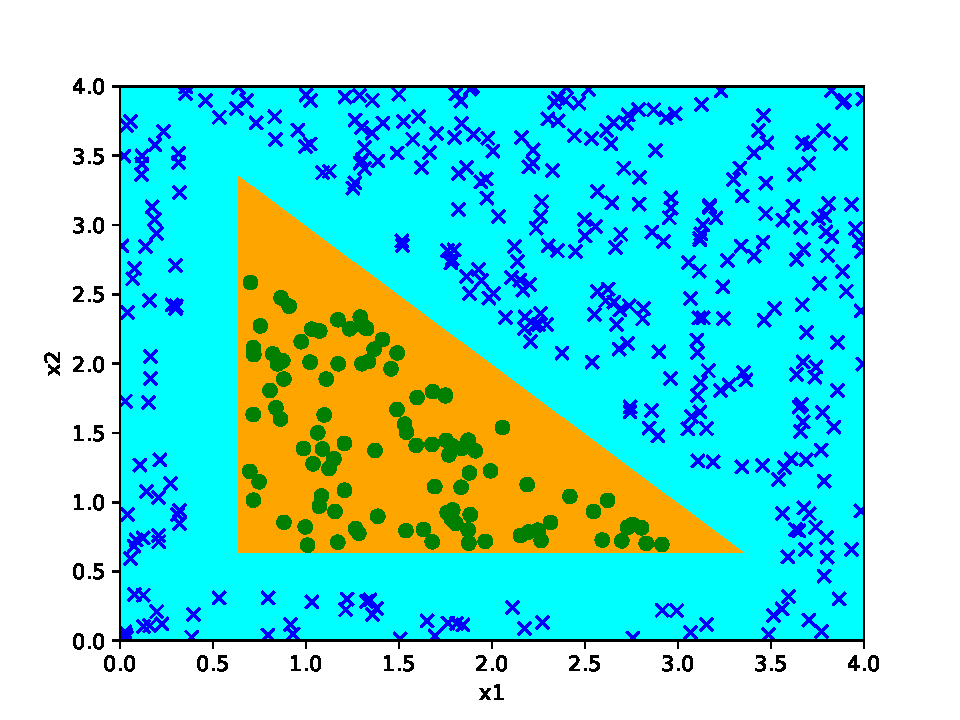
\includegraphics[width=0.6\textwidth]{src/simple_nn/step_weights.pdf}
        \caption{Decision Boundary -- Step activations}
    \end{figure}

\end{answer}
